\section{Оптмизации, проведенные в программе-симуляторе} % (fold)
\label{sec:ProgrammOptimisations}

    \subsection{Особенности многопоточной обработки данных} % (fold)
    \label{sub:MultithreadMulticoreDataProcessing}
        Широко известно, что увеличение тактовой частоты процессоров натолкнулось на физический предел, связанный с увеличением роли токов утечки в транзисторах при уменьшении размеров, и потому основной тренд в современном компьютеростроении - это наращивание числа ядер в процессорах, и улучшение эвристик, позволяющих использовать т.н. гиперпоточность. Итогом этого стала потенциальная возможность проводить вычисления в вплоть до 30-ти потоках одновременно, используя при этом только один процессор общего назначения (CPU).

        Когда речь идет о задачах молекулярной динамики, предполагается симуляция взаимодействия хотя-бы нескольких сотен тысяч частиц. По счастью, групповые явления наблюдаются и на гораздо меньшем масштабе - несколько (десятков) тысяч частиц.

        Свойство модели Vicsek'a, позволяющее успешно разбить задачу на множество потоков, ограниченное сверху лишь числом частиц заключается в том, что положения и скорости частиц в один момент времени однозначно определяют положения и скорости этих частиц в следующий момент. Также важно отметить, что это совершенно не зависит от порядка учета частиц. Таким образом, при разработке программы для выполнения на CPU мы можем безо всяких недостатоков получить практически линейное увеличение скорости вычислений в зависимости от доступного нам числа потоков.

        \begin{figure}[h]
        \centering
            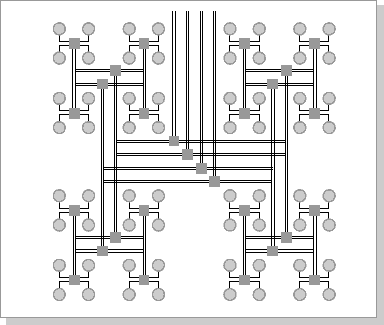
\includegraphics[height=200pt]{Images/KlusterArhitecture}
            \caption{Пример архитектуры вычислительного кластера}
            \label{fig:KlusterArchitecture}
        \end{figure}

        Задача несколько осложняется, если мы захотим пойти по пути всех исследовательских групп, и организовать выполнение приложения на вычислительном кластере. Поскольку, как мы видим на рис. \ref{fig:KlusterArchitecture}, между отдельными узлами кластера проложены связи по локальной сети, здравый смысл подсказывает, что доступ к общей памяти в такой архитектуре окажется куда медленней, чем если бы вся информация была доступна локально. Даже несмотря на возможность скопировать данные для вычислений на каждый из узлов, все равно требуется оптимизировать обмен данными после каждого шага.

        Кроме того, обычно очередность доступа к вычислительному кластеру жестко ограничивает возможность быстро исправить что-либо в программе и сразу же перезапустить ее для получения нового результата.
    % subsection MultithreadMulticoreDataProcessing (end)

    \subsection{GPGPU вычисления} % (fold)
    \label{sub:gpgpu}
        Проблема кластерных вычислений осложняется, помимо всего прочего, малой доступностью такого рода услуг. Здравый смысл подсказывает, что оборудование вычислительного кластера - сложный и дорогостоящий процесс, даже не принимая во вниамние дальнейшее обслуживание компьютерного парка. Потому, малым группам ученых без высокого финансирования необходимо искать обходные пути, не требующие доступа к кластерным суперкомпьютерам.

        \begin{figure}[h]
        \centering
            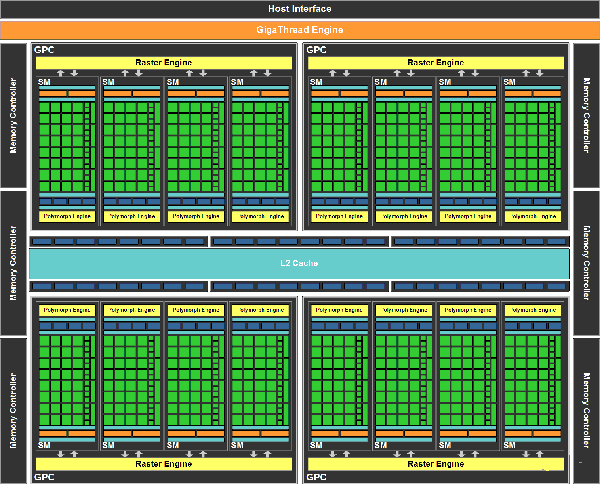
\includegraphics[height=200pt]{Images/GPU-diagramm}
            \caption{Пример архитектуры графического процессора}
            \label{fig:gpuArchitecture}
        \end{figure}

        Таким путем является использование графических процессоров для проведения вычислений общего назначения. Как показано на рис. \ref{fig:gpuArchitecture}, по существу графический процессор состоит нескольких сотен (или тысяч) простейших, т.н. потоковых процессоров, которые обладают поддеркой ограниченного набора инструкций, но при этом способных выполнять их действительно быстро. Кроме того, количество переходит в качество - простейшие вычисления, которые можно разбить на множество потоков могут выполняться одновременно всеми процессорами видеокарты.

        Также на диаграмме можно заметить, что процессори GPU, аналогично вычислительным юнитам в кластере, сгруппировани в ``вычислительные блоки'', с общим доступом к элементу памяти. Это позволяет проводить часть вычислений пользуясь локальной копией данных, а затем отправлять результаты в ``общий буфер'' - область памяти к которой имеют доступ все потоковые процессоры.

        В контексте модели Vicsek'a это позволяет нам, путем периодической сортировки частиц так, чтобы локально взаимодействующие частицы оказывались в смежной области памяти, существенно уменьшить число обращений к общей, и потому более медленной, памяти.
    % subsection gpgpu (end)

    \subsection{Определение равновестного состояния системы} % (fold)
    \label{sub:EquilibriumState}
        Помимо сугубо прикладных аспектов, т.е. вопроса ``на чем считать?'', необходимо отметить, что стандартная практика, применяемая во всех работах по моделированию самодвижущихся частиц, это запустить симуляцию для определенного значения шума, прождать от $10^{4}$ до $10^{6}$ шагов по времени, с тем чтобы ``минимизировать влияние начального распределения'', \cite{huepe2008}, и после этого заполучить результат. В некоторых работах, кроме того, производится усреднение интересующих значений по всему времени симуляции, к примеру в \cite{gregoire2004}.

        В условиях острой ограниченности вычислительных ресурсов, мы полагаем такой подход крайне расточительным. Потому, нами был предложен несложный алгоритм, позволяющий проводить симуляции столько, сколько потребуется для стабилизации значения интересующей нас величины, т.е. чтобы отклонения не превышали, в среднем, тех которые происходят под влиянием динамических флуктуаций. Подробнее этот алгоритм будет рассмотрен в разделе \ref{sec:StabilityAlgorithm}
    % subsection EquilibriumState (end)
% section ProgrammOptimisations (end)